%!TEX root = /Users/domaubert/Documents/Lectures/cosmolog/cosmo_main.tex

\chapter{l'Univers chaud}
Dans ce chapitre nous allons étudier de premières bases se rapportant à l'Univers quasi primordial âgé de quelques minutes au plus. Durant cette période, la dynamique de l'Univers est régie par les espèces relativistes, avec une dépendance temporelle du facteur d'expansion en $a(t)\sim\sqrt{t}$~: durant ces époques les influences respectives de la matière et de la constante cosmologique sont faibles. Ces premiers instants sont proches du Big-Bang et l'Univers s'y trouve dense et chaud~: ces conditions sont propices aux interactions entre atomes et particules subatomiques. C'est durant cette époque que les abondances des particules reliques\index{particule relique} et des éléments légers\index{element légers@élément légers}\sidenote{terme qui désigne les éléments de faible nombre de masse tels que H, He, Li ou Be} sont fixées~: c'est de ces abondances dont nous allons discuter dans ce chapitre.

\section{Équilibre \& Gel de réactions}
Les deux concepts fondamentaux des processus qui règlent les abondances\index{abondance} sont les notions \textit{d'abondance à l'équilibre}\index{abondance à l'équilibre} et de \textit{gel des réactions}\index{gel des réactions}. Dans notre cas, le terme d'abondance désigne la densité numérique d'une espèce atomique, subatomique, isotopique, etc. Par exemple l'abondance des atomes\index{atome} d'hydrogène se note $n_H$ et s'exprime en atomes par $m^3$. Les réactions qui permettent de modifier ces abondances font généralement intervenir d'autres réactifs. La photoionisation\index{ionisation} par exemple se caractérise par la réaction suivante:
\begin{equation}
n_H+\gamma \leftrightarrow n_{H+} + e^-,
\end{equation}
et dépend non seulement de l'abondance des atomes d'hydrogène\index{hydrogène} mais également de celle du nombre de photons\index{photon!UV} ionisants \sidenote{en l'occurrence surtout des photons ultra-violets}. Toutefois dans un très grand nombre de cas, la variation d'une espèce peut s'écrire comme ne dépendant que de sa propre abondance \textit{à l'équilibre} $n_e$ et d'un taux de réaction\index{taux de réaction} $\Gamma$ constant. Soit $n$ une abondance quelconque, son évolution pourra être suivie par une équation différentielle du type:
\begin{equation}
\frac{dn}{dt}=-\Gamma (n-n_e).
\end{equation}
Celle-ci est simple à comprendre. Si une abondance est déjà à l'équilibre\index{équilibre} $n=n_e$ et son abondance, par définition, ne varie pas. Si son abondance est supérieure à l'équilibre, le taux de réaction va agir comme une force de rappel\sidenote{on note que l'équation différentielle est similaire à celle décrivant la dynamique d'un ressort}, traduisant de fait une tendance à favoriser les réactions de destruction de l'espèce étudiée. À l'inverse si l'abondance est en déficit par rapport à l'équilibre, les réactions vont avoir tendance à la rétablir à des valeurs plus élevées. Notons que  l'inverse du taux de réactions fournit un temps caractéristique de retour à l'équilibre $t_e=\Gamma^{-1}$.

Toutefois il existe une autre manière de faire varier la densité numérique d'une espèce dans le contexte qui est le nôtre: il s'agit de la dilution cosmologique, déjà rencontrée dans le chapitre précédent. En effet, compte tenu de l'expansion de l'Univers\index{expansion}, si l'on dispose d'un certain nombre de particules d'un type donné dans un certain volume, sa \textit{densité} va évoluer même en l'absence de réactions (c'est-à-dire de destructions/créations). Ainsi la densité numérique d'une espèce donnée varie cosmologiquement de la façon suivante:
\begin{equation}
n=\frac{n_0}{a^3},
\end{equation}
ce qui ne fait que traduire l'équation différentielle suivante:
\begin{equation}
\frac{dn}{dt}=-3Hn,
\end{equation}
où $H$ est la fonction de Hubble usuelle \index{Hubble!fonction}, fonction du temps ou du paramètre d'expansion $H=\dot a/a$ \sidenote{le facteur 3 est typique de la dilution cosmologique d'une quantité \textit{volumique}, qui dépend du cube (donc à la puissance 3) de la longueur}. Comme déjà indiqué, le temps de Hubble\index{Hubble!temps} $t_H=H^{-1}$ fournit le temps caractéristique d'évolution significative des distances dans le cosmos.

Dans le cas cosmologique général, les deux procédés se superposent et l'abondance d'une espèce arbitraire est régie par une équation de type:
\begin{equation}
\frac{dn}{dt}=-3Hn-\Gamma (n-n_e).
\label{e:reac}
\end{equation}
Cette équation demande en toute généralité à être résolue numériquement. Toutefois 2 cas limites se détachent facilement:
\begin{itemize}
\item si $H\gg \Gamma$ : l'expansion est beaucoup plus efficace que les réactions. C'est un régime où le second terme de l'équation \ref{e:reac} peut être négligé, on retrouve $n\sim a^{-3}$ et le nombre de particules dans un volume en expansion donné est \textit{constant}. On dit que l'espèce est \textit{gelée}.
\item si $H\ll \Gamma$ : on peut négliger la dilution cosmologique et les temps de retour à l'équilibre sont très courts. L'abondance est celle de l'équilibre, qui est éventuellement une fonction du temps $n\sim n_e(a)$.
\end{itemize}

En règle générale $H$ et $\Gamma$ sont tous deux fonctions du temps et $\Gamma$ a tendance à dominer au début de l'histoire de l'Univers (quand les densités et températures sont très élevées) pour être ensuite dominé par $H$. En effet à ces époques, la dynamique est dominée par le rayonnement et 
\begin{equation}
H\sim\frac{1}{a^2}
\end{equation}
tandis qu'un taux de réaction est du type $\Gamma\sim \sigma v n$ où $v\sim a^{-i}$ est une vitesse typique des réactifs, $\sigma$ une section efficace et $n\sim a^{-3}$ une densité volumique de réactifs. En supposant une section efficace de réaction constante, on a une dépendance de $\Gamma$ en facteur d'expansion $a$ qui est au moins de l'ordre de :
\begin{equation}
\Gamma \sim \frac{1}{a^{3+i}}.
\end{equation}
La vitesse décroit avec la température, dont on verra qu'elle décroît avec le paramètre d'expansion $a$ et donnant $i>0$ : les taux de réactions dépendent plus fortement de l'histoire d'expansion pour dominer puis être dominés par $H$ au cours de la croissance de $a$. Par conséquent l'histoire typique de l'abondance d'une espèce suit d'abord celle de l'équilibre avant d'être gelée et n'être plus modifiée que par la dilution cosmologique. Cette transition porte le nom de «gel» ou \textit{freeze-out} en anglais\index{gel des réactions}.



\section{Statistique d'un gaz}
La question qui se pose à présent est celle de déterminer l'abondance à l'équilibre d'une espèce (hydrogène, photons, neutrinos, etc..). Celle-ci nous est donnée par la physique statistique\index{statistique d'un gaz}.

On se place dans le cas simple d'une particule libre\index{particule libre}\sidenote{non soumise à un potentiel extérieur}, auquel cas son énergie ne dépend que de son impulsion $\vec p$, ou bien de façon équivalente que de son vecteur d'onde\index{vecteur d'onde} $\vec k =\vec p /\hbar$ \sidenote{ici $\hbar=\frac{h}{2\pi}$ désigne la constante de Planck réduite}:
\begin{equation}
E^2=p^2c^2+m^2c^4=\hbar^2 c^2 k^2 +m^2c^4.
\end{equation}
 Plus précisément l'énergie d'une particule ne dépend que de la norme $k$ du vecteur d'onde\index{nombre d'onde}. Par conséquent, l'ensemble des points dans l'espace des $\vec k$ qui fournissent une énergie donnée sont à l'intérieur d'une coquille de rayon $k$. De plus, le peuplement de cet espace est quantifié : en effet les nombres d'ondes accessibles (c.-à-d. les impulsions accessibles) doivent être de la forme $\vec k = (n_x,n_y,n_z) 2\pi/L $ où $L$ désigne la taille de la «cuve» dans laquelle s'effectue l'étude et où le triplet est un triplet de valeurs entières. Par conséquent, une particule ne peut se trouver que sur les nœuds d'une maille pavant cet espace. 

Ces considérations nous permettent d'évaluer le \textit{nombre d'états accessibles à une énergie E donnée}\index{nombre d'états}. Ce nombre est donné par le rapport entre le volume de l'espace des $\vec k$ à énergie $E$ donnée (la coquille):
\begin{equation}
4\pi k^2 dk
\end{equation} 
et le volume occupé par un état unique (le volume de la maille):
\begin{equation}
(2\pi/L)^3.
\end{equation}
On obtient alors le nombre d'états accessible à une particule libre d'énergie $E$ à $dE$ près \index{densité d'états}
\begin{equation}
N(E)dE=\frac{4\pi k^2 dk}{(2\pi/L)^3}.
\label{e:densetat}
\end{equation}

\begin{figure}[htbp]
	\centering
		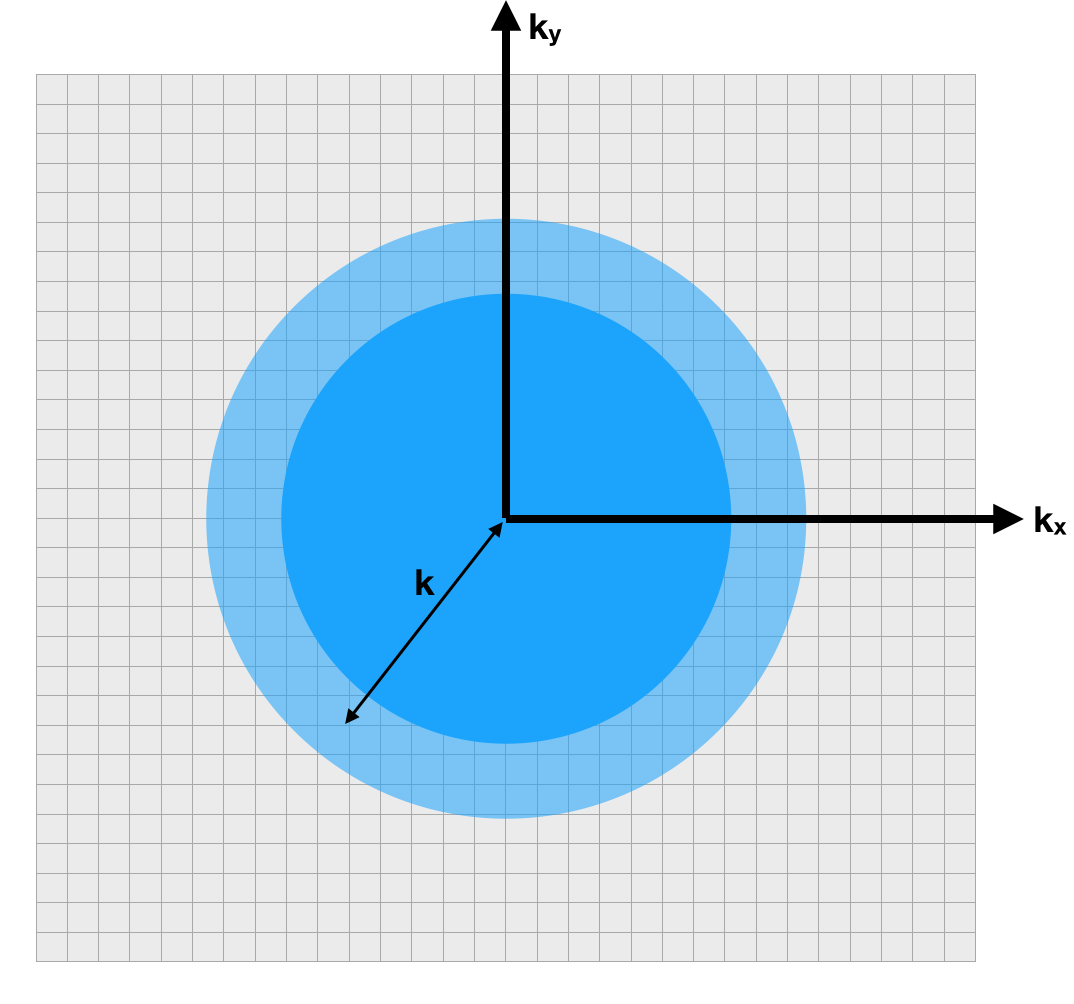
\includegraphics[height=12cm]{figs/k.png}
	\caption[Calcul de la densité d'états libres]{Comment calculer le nombre d'états d'énergie donnée ? Les états sont quantifiés et «positionnés» sur une maille correspondant à des valeurs de $k_x$ et $k_y$ multiples de $2\pi/L$. Tous les états de même énergie partagent le même module $k$ : leur nombre est donc donné par la surface de la coquille ($2\pi k dk$) divisée par la surface d'un élément de la maille ($(2\pi/L)^2$). À 3D, ce nombre devient $4 \pi k^2 dk / (2\pi/L)^3$.}
	\label{f:k}
\end{figure}

L'équation \ref{e:densetat} n'est pas suffisante pour calculer l'abondance d'une particule: elle nous renseigne sur la quantité d'états accessible mais reste à déterminer combien de particules résident sur un état donné. Le \textit{niveau d'occupation}\index{niveau d'occupation d'un état} dépend du type de particule: si celle-ci est un fermion\index{fermion}\sidenote{une particule dont le spin est demi-entier comme l'électron ou  le proton} alors elle est soumise au principe d'exclusion de Pauli qui stipule qu'un état quantique donné ne peut être occupé, au plus, que par une particule. Si celle-ci est un boson\index{boson}\sidenote{une particule dont le spin est entier, comme le photon}, cette restriction ne s'applique pas. Plus précisément, les niveaux d'occupation sont donnés par les statistiques de Fermi-Dirac\index{Fermi-Dirac} et Bose-Einstein\index{Bose-Einstein}
\begin{equation}
n(E)=\frac{g(E)}{\exp(\beta(E-\mu))\pm 1}.
\label{e:BEFD}
\end{equation}
Le signe positif (resp. négatif) au dénominateur désigne la statistique de Fermi-Dirac\index{Fermi-Dirac!statistique} (resp. Bose-Einstein \index{Bose-Einstein!statistique}).La quantité $\beta=1/k_B T$ dépend est une représentation de la température\index{température}, $\mu$ est le potentiel chimique\index{potentiel chimique} de l'espèce étudiée et $g(E)$ est la dégénérescence\index{dégénérescence} d'un état d'énergie $E$. Cette dernière quantité dépend également de la particule considérée. On note que dans le cas d'une statistique de Fermi-Dirac, s'appliquant aux fermions, $n(E)\le g(E)$\sidenote{avec un dénominateur supérieur à 1}: cela découle du principe d'exclusion de Pauli\index{principe d'exclusion} l'occupation est au mieux égale à la dégénérescence du niveau d'énergie. À l'inverse les bosons, soumis à la statistique de Bose-Einstein, peuvent avoir des niveaux d'occupation arbitrairement grands.

À ce stade, l'abondance d'une particule peut être déterminée et le nombre total de particules d'une espèce donnée dans une cuve de volume $V=L^3$ à température $T$ est
\begin{equation}
N=\int_{E_{\mathrm{min}}}^\infty n(E)N(E) dE.
\label{e:abondance}
\end{equation}
Notons que cette intégrale porte sur toutes les énergies, depuis la plus faible jusqu'aux infinis. Cette valeur plancher de l'énergie dépend de la particule considérée. Par exemple pour une particule de masse nulle\sidenote{tel le photon}, on aura $E_\mathrm{min}=0$ tandis que pour une particule massive on aura $E_\mathrm{min}=mc^2$, correspondant à un état de repos (et donc d'impulsion minimale) absolu.

\section{Les photons}
Le cas des photons\index{photon} permet d'illustrer le calcul de la section précédente tout en étant d'une grande pertinence cosmologique: ils appartiennent aux particules dites relativistes et c'est elles qui dominent le budget numérique actuel de l'Univers. 

Le calcul de l'abondance des photons nécessite de préciser d'abord les quelques nombres nécessaires à sa bonne conduite. Dans un premier temps, les photons sont des particules de masse nulle, donc leur énergie est faite d'impulsion pure:
\begin{equation}
E_\gamma=pc=\hbar c k.
\end{equation} 
On rappelle que la densité d'états accessibles possédant une norme $k$ donnée a pour expression 
\begin{equation}
\frac{N(k)dk}{V}=\frac{4\pi k^2 dk}{V}\left(\frac{L}{2\pi}\right)^3=\frac{4\pi (E/\hbar c)^2 dE}{\hbar c V}\left(\frac{L}{2\pi}\right)^3.
\end{equation}
Par conséquent la densité volumique d'états d'énergie E accessible aux photons est donnée par:
\begin{equation}
\frac{N(E)dE}{V}=\frac{1}{2\pi^2}\frac{E^2dE}{(\hbar c)^3}.
\end{equation}
De plus le photon est sa propre antiparticule\index{antiparticule} et participe par exemple aux équations de désintégrations:
\begin{equation}
A + \bar{A} \leftrightarrow \gamma+\gamma.
\end{equation}
Or $\mu_A=-\mu_{\bar{A}}$ donc $\mu_\gamma=0$. Enfin le photon autorise deux hélicités par état d'énergie et possède un spin entier et obéit donc à la statistique de Bose-Einstein\index{Bose-Einstein!statistique}. L'état d'occupation d'un niveau d'énergie E est donc donné par :
\begin{equation}
n(E)=\frac{2}{e^{\frac{E}{k_B T}}-1}.
\end{equation}
D'où son abondance à l'équilibre:
\begin{equation}
n_\gamma=\frac{1}{(\hbar c)^3\pi^2}\int_0^\infty\frac{E^2dE}{e^{\frac{E}{k_B T}}-1}.
\end{equation}
On reconnait dans l'intégrale la distribution de Planck\index{Planck!distribution}, qui par définition décrit la distribution spectrale d'énergie d'un gaz de photons à l'équilibre, comme présent par exemple dans un corps noir\index{corps noir}. Cette intégrale peut être conduite analytiquement conduisant à \sidenote{en utilisant l'expression de la fonction \textit{zêta} de Riemann avec $\zeta(3)=\frac{1}{\Gamma(3)} \int_0^\infty \frac{x^2}{e^x-1}dx$.} :
\begin{equation}
n_\gamma \approx 0.244 \left(\frac{k_BT}{\hbar c}\right)^3 \mathrm{m}^{-3}.
\label{e:densphot}
\end{equation}

Aujourd'hui la température\index{température!gaz de photons} du gaz de photons du cosmos est de l'ordre de 2.73 K, correspondant à une densité de photons actuelle de :
\begin{equation}
n_\gamma\approx 410 \mathrm{cm}^{-3}.
\end{equation}
Pour mémoire, la densité d'atomes d'hydrogène\index{hydrogène!densité} actuelle (espèce qui domine la population de baryons) est de l'ordre de l'atome par $m^3$, on est donc dans un rapport de $10^{8-9}$,  extrêmement en faveur des photons. Une évaluation plus précise du rapport baryon/photon\index{rapport baryon/photon} $\eta$ est donnée par:
\begin{equation}
\eta \approx 5\times 10^{-10}\frac{\Omega_b h^2}{0.02}
\end{equation}
Cette surabondance de lumière résulte du processus de désintégration des particules massives que nous étudierons par la suite. 

\section{Histoire de la température}

Si l'on examine à nouveau l'expression de la densité de photon (Éq. \ref{e:densphot}), on constate que celle-ci varie en $n_\gamma \sim T^3$\index{photon!densité}. Ainsi si l'on considère une cuve de volume $V$ elle contient à un redshift $z$ donné le nombre de photons suivant:
\begin{equation}
N_\gamma(z) \sim V(z) T(z)^3.
\end{equation}
Or compte tenu de leur gigantesque domination numérique, ce nombre de photons doit être \textit{constant}: aucun processus (absorption/émission, à priori par des baryons extrêmement peu nombreux par rapport aux photons) ne peut changer $N_\gamma$ de façon significative. Toutefois, une cuve de taille donnée verra ses limites évoluer sous l'effet de la dynamique de l'Univers. En particulier $V=V_0 a^3$ d'où la loi d'évolution de la température des photons\index{température!photon}
\begin{equation}
T_\gamma=\frac{T_0}{a}=T_0 (1+z),
\end{equation}
avec $T_0=2.73K$. De plus compte tenu de la domination quasi totale des espèces relativistes sur le bilan numérique des particules du cosmos (comme illustrée par la valeur de $\eta$), on peut presque considérer que cette température est celle du cosmos. 

Une autre démonstration de cette relation repose sur le fait que le spectre doit conserver sa forme de courbe de Planck\index{Planck!distribution}, y compris sous l'effet de l'expansion, car c'est effectivement ce qui est observé aujourd'hui. Or le nombre de photons qui tombe dans une bande d'énergie $dE$ est, à une constante multiplicative près\sidenote{avec $V=a^3 V_0$ et $E=\frac{E_0}{a}$.},
\begin{equation}
V \frac{E^2 dE}{e^{\frac{E}{k_B T}}-1}=V_0 \frac{E_0^2 dE_0}{e^{\frac{E_0}{k_B aT}}-1}.
\end{equation}
Pour que le spectre reste inchangé, il faut «neutraliser» la dernière dépendance en $a(t)$ qui se trouve dans le terme de l'exponentielle, en imposant que $a(t) T$ reste constant, redonnant ainsi l'expression précédente.


Aujourd'hui l'Univers est froid, mais par le passé celui-ci était plus chaud, en plus d'être plus dense comme expliqué dans les chapitres précédents. Notons pour finir que les photons du cosmos ne sont plus à l'équilibre thermodynamique à proprement parler depuis la production du fond diffus cosmologique\index{fond diffus cosmologique} : aujourd'hui ces photons n'interagissent plus avec les baryons, interactions qui auraient permis de maintenir le bain de photons à l'équilibre. Toutefois dans le passé plus chaud et plus dense, ces interactions existaient et un régime de fort couplage permettait de garantir un couplage matière rayonnement suffisant pour que la situation «thermodynamique» de l'Univers s'apparente à celle d'un corps noir\index{corps noir}. Cette situation a cessé (380 000 ans après le Big Bang comme nous le verrons) mais la domination des espèces relativistes est telle qu'aucun processus n'est en mesure de changer significativement la fonction de distribution des photons: en l'absence de processus permettant cette modification, le gaz de photons a pu conserver la mémoire d'une période antérieure d'équilibre thermodynamique\index{équilibre!thermodynamique}.

Par la suite nous considèrerons des époques durant lesquelles le bilan énergétique de l'Univers est dominé par les espèces relativistes durant lesquelles le facteur d'expansion varie en :
\begin{equation}
a\sim \sqrt t.
\end{equation}
Il en découle les lois d'échelles suivantes \sidenote{on rappelle que le MeV désigne 1 million d'électrons-volts et constitue une énergie équivalente à $1 MeV \sim 1.6 \times 10^{13} J$}:
\begin{equation}
T\approx\frac{10^{10} K}{\sqrt{t\mathrm{(sec)}}} \approx \frac{1}{k_B}\frac{1 \mathrm{MeV}}{\sqrt{t\mathrm{(sec)}}}.
\end{equation}
Ces lois permettent déjà de se faire une idée des hautes températures en place durant les phases primordiales de l'Univers et donc permettent d'anticiper que des processus très énergétiques sont en mesure d'être effectifs. Par exemple les énergies typiques du LHC\index{LHC} sont de l'ordre du TeV $=10^6$ MeV: elles correspondent aux énergies typiques dans un Univers de $10^{-12}$ secondes. De plus ces lois d'échelles permettent d'anticiper que certaines époques joueront un rôle pour certaines particules quand l'énergie typique du cosmos est de l'ordre de leur énergie de masse : par exemple l'électron\index{electron@électron} possède une énergie de masse proche du MeV ( 511 keV exactement) et donc il est probable que son abondance soit significativement modifiée lorsque l'Univers aura un âge correspondant à cette masse (à savoir de l'ordre de la seconde).


\section{Évolution des abondances}
Pour une «particule» quelconque, l'expression précise de son abondance\index{abondance} va dépendre de son caractère relativiste ou non. Il existe des particules pour lesquelles ce caractère reste inchangé au cours du temps, comme les photons par exemple, mais en général, une particule aura tendance à être considérée comme relativiste aux premiers instants de l'Univers puis évoluera plus tard vers le régime non relativiste, avec comme conséquence une variation, parfois radicale, de son abondance au cours du temps.

L'énergie d'une particule libre\index{particule libre} est donnée par :
\begin{equation}
E=\sqrt{p^2c^2+m^2c^4}.
\end{equation}
 Une particule est dite \textit{ultra-relativiste}\index{particule!ultra-relativiste} si son énergie de masse\index{energie@énergie!masse} est considérée comme négligeable devant son énergie cinétique\index{energie@énergie!cinétique}, $pc\gg mc^2$, auquel cas $E\sim pc$. C'est notamment le cas du photon, étudié en détail dans la section précédente. À l'inverse, une particule est dite \textit{non-relativiste}\index{particule!non-relativiste} si son énergie de masse constitue l'essentiel de son énergie totale $pc \ll mc^2$. Cela correspond au fluide «matière» développé dans le chapitre précédent et dans ce cas $E\sim mc^2 (1+ p^2/2m) \sim mc^2$. L'utilisation de l'une ou l'autre de ces expressions pour l'énergie dans l'équation \ref{e:abondance} va conduire à des expressions différentes des abondances.
 
 \paragraph{Cas ultra-relativiste\index{particule!ultra-relativiste}}
Ce cas correspond à celui étudié précédemment pour les photons : en effet, si l'on parle du principe que la masse d'une particule est négligeable, elle en devient quasi similaire à un photon et son abondance n'en diffère que par le facteur de dégénérescence et par la statistique à utiliser (BE ou FD). En conséquence, l'abondance d'une particule dans ce régime ultra-relativiste sera proche de celle des photons. Un calcul précis donne l'abondance suivante pour un \textit{boson}\index{boson}
\begin{equation}
n_B=n_\gamma\frac{g_B}{2},
\end{equation}
tandis que si la particule étudiée est un fermion\index{fermion}
\begin{equation}
n_F=n_\gamma\frac{3g_F}{8}.
\end{equation}
À un facteur proche de l'unité près, l'abondance d'une particule relativiste est essentiellement celle des photons $n\sim n_\gamma$.

\paragraph{Cas non relativiste\index{particule!non-relativiste}}
Dans ce régime, l'énergie d'une particule est la somme de l'énergie cinétique classique et de son énergie de masse, $E\sim p^2/2m +mc^2$ et l'occupation statistique des énergies (cf. éq. \ref{e:BEFD}) devient la statistique de  Maxwell-Boltzmann\index{Maxwell-Boltzmann!statistique}, donnée par\sidenote[][-3cm]{généralement cette statistique devient valable quand $e^{\frac{\min{E}-\mu}{k_B T}}\ll 1$. Or on verra ci-dessous que ce régime non relativiste est précisément décrit par une température faible devant l'énergie de masse $k_BT \ll mc^2$ avec $\min E =mc^2$}:
\begin{equation}
g e^{-\frac{E-\mu}{k_B T}}.
\end{equation}
 L'abondance est alors donnée par l'expression suivante 
\begin{equation}
n=\frac{g}{2\pi^2 \hbar^3}e^{-\frac{mc^2-\mu}{k_BT}}\int_0^\infty p^2 e^{-\frac{p^2}{2mk_B T}}dp.
\end{equation} 
 Le calcul de son abondance donne une quantité qui dépend directement de la température\index{température}\sidenote{on note que l'intégrale porte sur $\infty$ alors qu'elle devrait être bornée pour satisfaire l'hypothèse non relativiste. Toutefois, l'intégrande est une gaussienne dont la décroissance est très rapide : l'erreur est donc faible et permet de reconnaître l'expression de la (moitié de la) variance d'une distribution normale.}
\begin{equation}
n=ge^{\frac{\mu}{k_BT}}\left(\frac{m k_B T}{2\pi\hbar^2}\right)^{3/2}e^{-\frac{mc^2}{k_B T}}\sim e^{-\frac{mc^2}{k_B T}}.
\label{e:nonrel}
\end{equation}


Compte tenu de l'évolution de la température, qui décroit avec le temps, l'abondance décroît de façon exponentielle. La réaction typique permettant cette décroissance est une réaction de \textit{désintégration}:
\begin{equation}
A+\bar A \leftrightarrow \gamma+\gamma,
\end{equation}
avec un déplacement de l'équilibre vers la droite de cette équation, c.-à-d. vers le réservoir de photons.

\paragraph{Transition}
Se pose alors la question de la détermination du régime dans lequel se trouve une particule. Il s'avère que la température d'un gaz de particule est liée à l'énergie cinétique et $E_c\sim k_B T$. Par conséquent à haute température, $k_B T\gg mc^2$, une particule tend à être ultra-relativiste\sidenote{on a la vitesse $v\sim\sqrt{k_B T}$ qui tend à devenir non-négligeable devant $c$.} tandis qu' à basse température $k_B T\ll mc^2$, celle-ci tend à être non relativiste. On sait également que la température de l'Univers décroît au cours du temps, donc pour une particule massive donnée, il se trouvera toujours une époque reculée où cette particule est relativiste, suivie par une époque où elle basculera dans le régime non relativiste. La transition entre les deux régimes opère lorsque l'énergie cinétique typique est de l'ordre de l'énergie de masse\index{energie@énergie!masse}
\begin{equation}
k_B T(z^*)=mc^2.
\end{equation}
Sachant que la température du rayonnement\index{température!rayonnement} varie en $T_\gamma\sim (1+z)$ et qu'à l'équilibre un fort couplage existe, la transition opère à un redshift $z^*$ donné par :
\begin{equation}
1+z^*=\frac{mc^2}{k_B T_0}.
\end{equation}
 On constate ainsi qu'une particule passera dans le régime non relativiste d'autant plus rapidement qu'elle sera massive. À l'inverse, une particule de masse nulle ne pourra jamais, comme attendu, basculer dans le régime non relativiste.
 

 
 \section{Abondances résiduelles}
 
\begin{figure}[htbp]
	\centering
		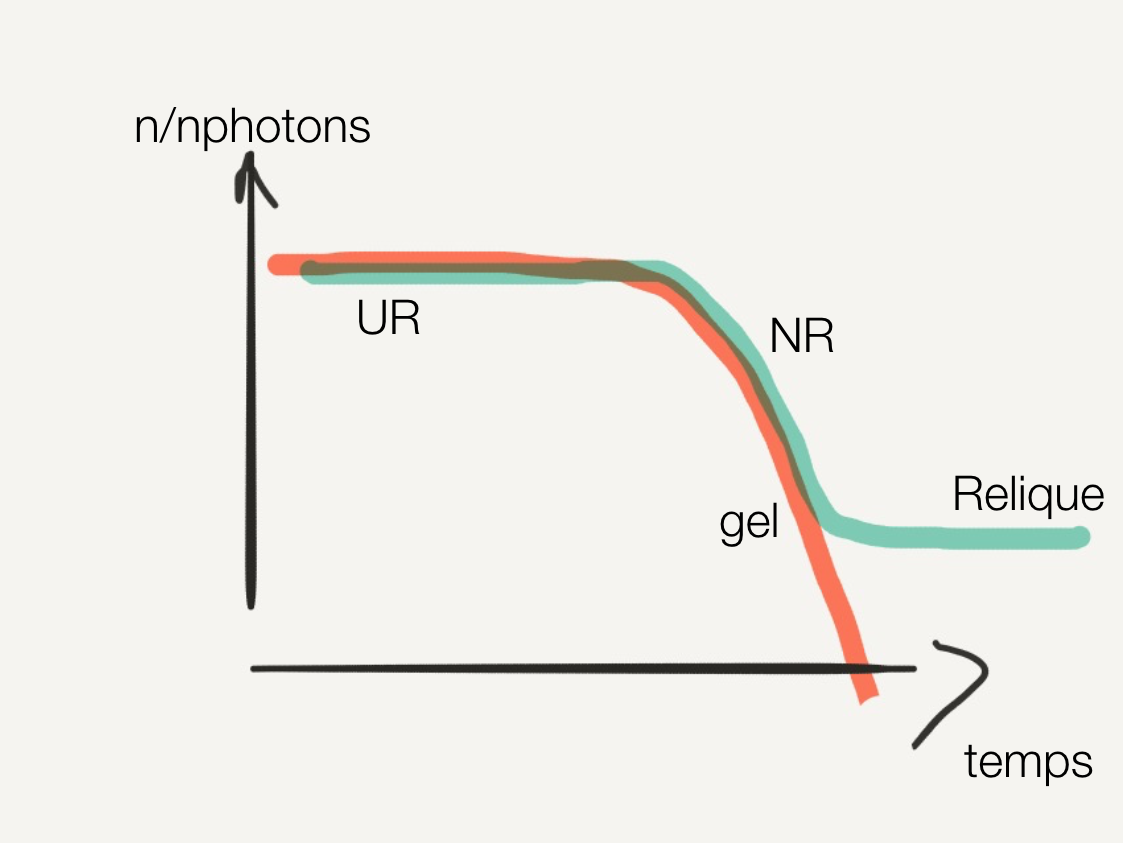
\includegraphics[height=12cm]{figs/freeze.png}
	\caption[Évolution schématique de l'abondance d'une particule relique.]{Évolution schématique de l'abondance d'une particule relique. Dans le régime ultra-relativiste (UR), la particule se comporte comme un photon et son abondance est similaire. Le passage au régime non relativiste (NR) provoque la décroissance de l'abondance, exponentielle, typique d'une particule massive. Son abondance deviendrait négligeable sans le «gel» (freeze-out)~: la dilution cosmologique ainsi que l'absence de réactifs ou la baisse de température vont stabiliser la densité numérique de la particule à une abondance non nulle. }
	\label{f:freeze}
\end{figure}
 
 
  En résumé, l'abondance\index{abondance!à l'équilibre} à l'équilibre d'une particule passe par 2 étapes distinctes:
 \begin{itemize}
 \item à grand $z>z^*$, nous avons $k_B T \gg mc^2$ et $n\sim n_\gamma$
 \item à bas  $z<z^*$, nous avons $k_B T \ll mc^2$ et l'abondance décroît de façon exponentielle. Elle se désintègre et son abondance devient très inférieure à l'abondance des photons, $n\ll n_\gamma$.
 \end{itemize}
Or nous avons vu précédemment que les réactions qui permettent le maintien de cet équilibre vont «geler» \index{gel des réactions}\sidenote{appelé aussi \textit{Freeze-out}} et peuvent découpler une espèce de la «soupe» de particules en interaction: après ce gel, l'abondance d'une espèce va rester celle de l'équilibre au moment du découplage. Ce gel peut opérer avant ou après $z^*$. Si une particule gèle pour $z>z^*$, elle se trouvait dans son régime relativiste, en grande abondance. Une particule de ce type va rester très abondante jusqu'à nos jours et c'est par exemple le cas des neutrinos\index{neutrinos}. Si à l'inverse elle gèle pour $z<z^*$, alors celle-ci avait déjà entamé sa désintégration durant laquelle son abondance décroît de façon exponentielle. Par conséquent la particule est en très faible abondance et aujourd'hui son abondance doit être très faible devant celle des photons (et donc des neutrinos). C'est le scénario essentiellement de toutes les particules massives, que l'on appelle aussi \textit{particules reliques}\index{particules reliques} car elles auront survécu à ce processus.
 
 \section{Asymétrie Matière-Antimatière\index{asymétrie matière-antimatière}\index{antimatière}}
Pour conclure ces considérations sur la physique de l'Univers chaud et énergétique, quelques mots sur l'asymétrie matière-antimatière. Les baryons ont un nombre quantique baryonique de valeur +1 et on peut leur associer des \textit{antibaryons}, de nombre baryonique -1 : le proton et le neutron possèdent ainsi des antibaryons que sont l'antiproton et l'antineutron \sidenote{dans le cas de l'antiproton, cela se manifeste notamment par une charge électrique opposée et donc négative}. Au-delà de ces considérations sur ces nombres quantiques, l'assemblage d'antibaryons permet de faire de l'antimatière qui en tout autre point ressemble beaucoup à la matière normale : ces 2 types opposés partagent par exemple la même masse et toute réaction de type matière peut en principe être réalisée dans sa version antimatière \sidenote{on parle de réaction conjuguée}.

Lorsque les particules reliques sont en phase de désintégration et voient leurs abondances chuter de façon exponentielle, l'un des canaux privilégiés de cette baisse est précisément le processus d'annihilation\index{annihilation} matière-antimatière. Soit une particule $A$ et son antiparticule $\bar A$, leur éventuelle rencontre conduit à la production d'énergie pure sous forme de photons:
\begin{equation}
A+ \bar A \leftrightarrow \gamma.
\end{equation}
 Ce processus est extrêmement efficace et on peut montrer qu'en cas d'abondance initiale égale entre particules et antiparticules, l'abondance des particules reliques devrait être de l'ordre de :
 \begin{equation}
 \eta=\frac{n_B}{n_\gamma}\sim10^{-18}.
 \end{equation}
 Or nous venons de voir que l'ordre de grandeur observé actuellement du rapport baryons sur photons $\eta\sim10^{-9}$ est environ $10^9$ plus grand. Ceci suggère fortement que le gel des abondances des baryons a été dicté par l'absence de réactifs de type antibaryons plutôt que par une perte d'efficacité de la réaction, avec un excès en faveur de la matière de l'ordre de :
 \begin{equation}
 \frac{n_A-n_{\bar A}}{n_A+n_{\bar A}}\sim10^{-9}.
 \end{equation}
 Par ailleurs, nous constatons autour de nous une absence d'abondance significative d'antimatière, qui autrement se manifesterait par la production de photons gamma à très haute énergie lors de rencontre avec la matière \sidenote{les photons produits par les annihilations emportent une énergie $mc^2$, donc de l'ordre du GeV pour des protons-antiprotons par exemple.} Tout indique qu'il existait une asymétrie dans les abondances initiales de particules et d'antiparticules, faible mais non nulle et suffisante pour que notre Univers soit aujourd'hui dominé par la matière.
 
Ceci étant posé, comment expliquer une telle asymétrie ? Une première possibilité est qu'il s'agisse simplement d'une des caractéristiques de notre Univers. Une seconde possibilité est qu'il existe des mécanismes qui sont capables de transformer une situation initialement symétrique en situation présentant une légère surabondance de matière : ces processus auraient été à l'œuvre lors d'un évènement que l'on nomme la \textit{Baryogénèse}\index{Baryogénèse}. Aujourd'hui, nous ne savons pas quand elle a eu lieu\sidenote{si elle a eu lieu} et sous quelles modalités exactes. Par contre dès 1967, Sakharov posa 3 conditions\index{conditions de Sakharov} qui doivent être satisfaites à minima pour que la Baryogénèse ait pu prendre place :
\begin{enumerate}
\item il faut des réactions qui ne conservent pas le nombre baryonique:
\begin{eqnarray}
A + \bar B &\leftrightarrow& C
\end{eqnarray}
C'est une condition minimale pour qu'une situation symétrique puisse évoluer vers une asymétrie.
\item il faut que les réactions conjuguées aient des taux de réactions différents.
\begin{eqnarray}
A + \bar B &\leftrightarrow& C\\
\bar A + B &\leftrightarrow& \bar C.
\end{eqnarray}
En effet, pour une réaction qui ne conserve pas le nombre baryonique, la réaction conjuguée est également possible : si elles sont toutes aussi efficaces, le nombre baryonique global reste nul et la symétrie n'est pas brisée.
\item si les 2 conditions précédentes sont réalisées, nous obtenons une population en $C$ et $\bar C$ asymétrique. Toutefois, il ne faut pas que l'équilibre thermodynamique soit maintenu : comme vu précédemment l'abondance d'une particule à l'équilibre ne dépend que de sa masse, qui est identique pour les 2 types de matière. Il faut figer le déséquilibre créé et par exemple empêcher que nos réactions puissent retourner à l'état initial symétrique:
\begin{eqnarray}
A + \bar B &\rightarrow& C\\
\bar A + B &\rightarrow& \bar C.
\end{eqnarray}
\end{enumerate}
\begin{figure}[htbp]
	\centering
		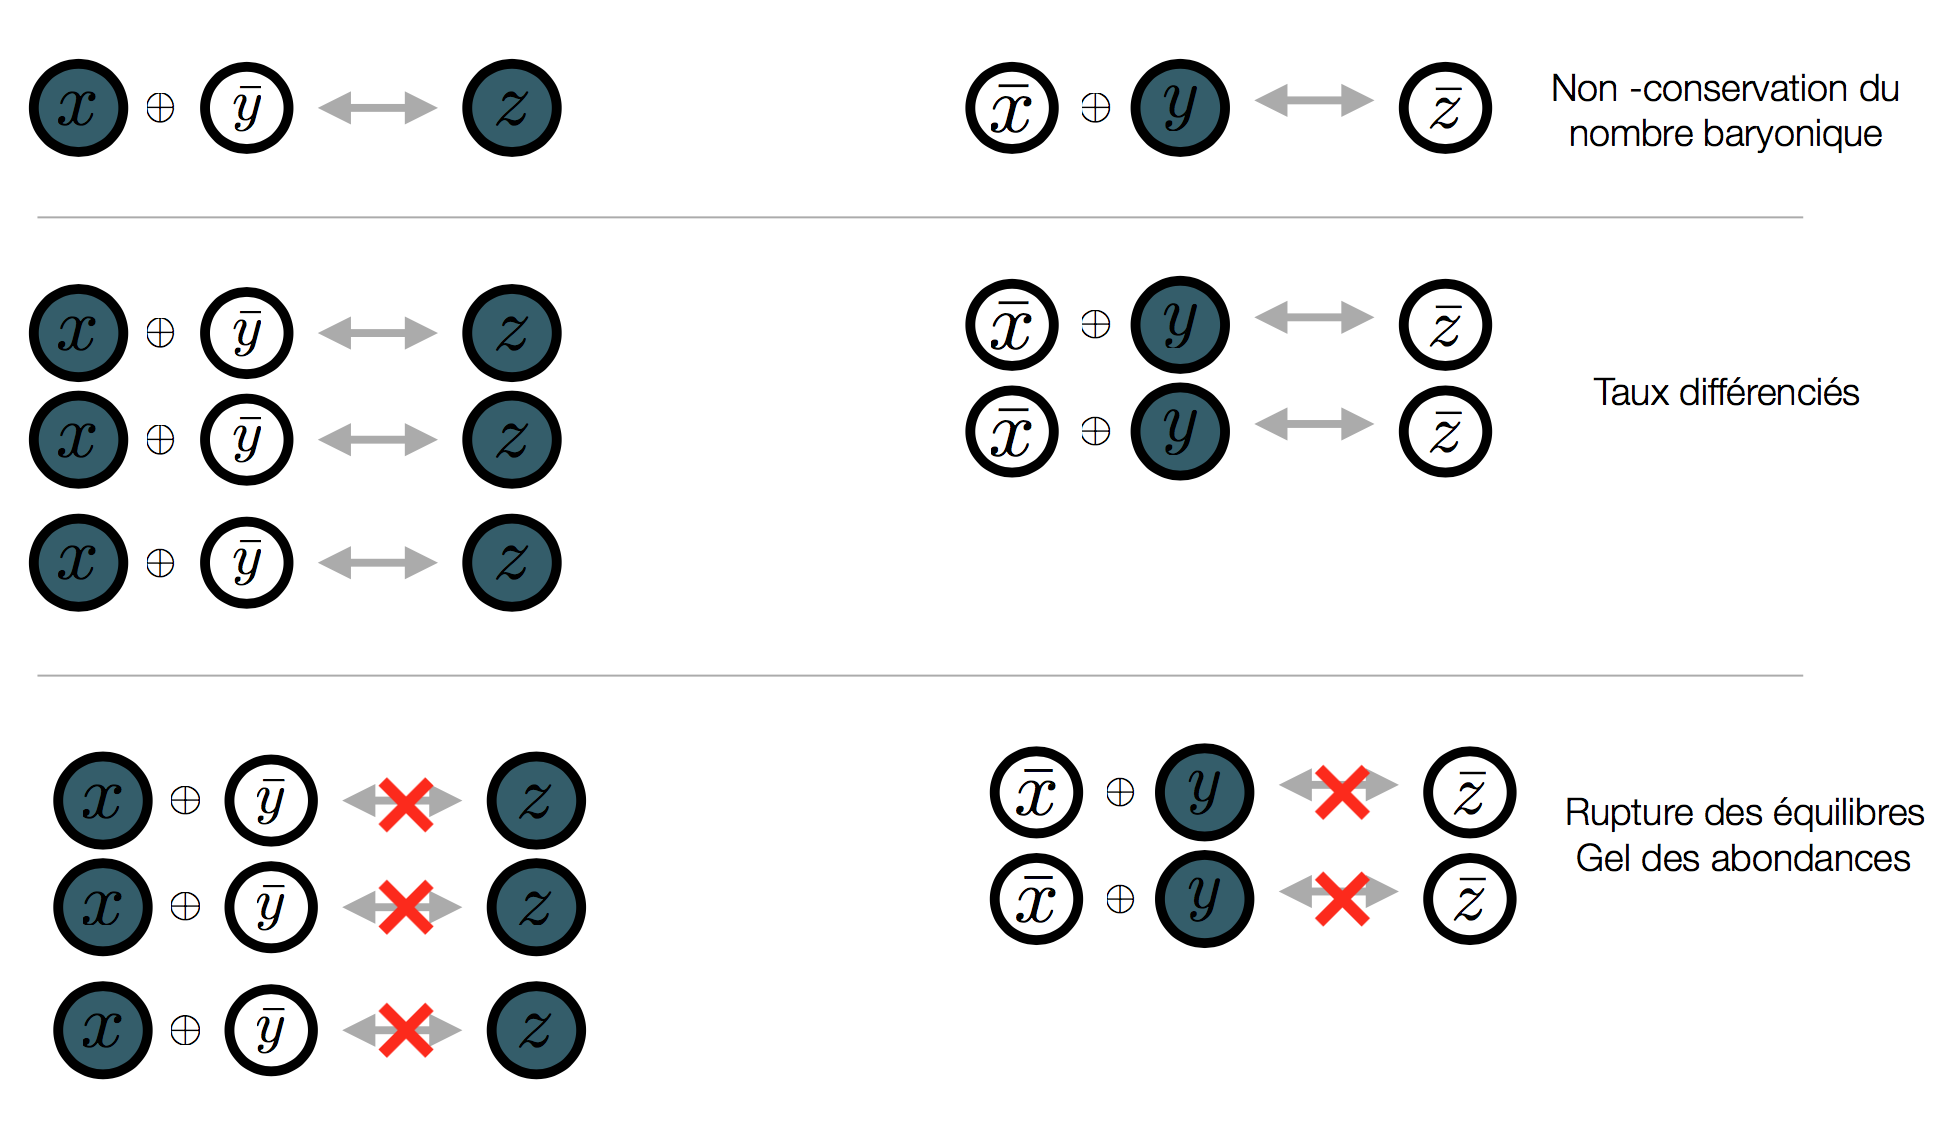
\includegraphics[height=12cm]{figs/sakharov.png}
	\caption[Les conditions de Sakharov][-2cm]{Les conditions de Sakharov, nécessaires à l'existence d'une Baryogénèse à l'origine de l'asymétrie matière-antimatière. Il faut des réactions qui ne conservent pas le nombre de baryons, qui opèrent à des taux différents quand elles sont réalisées avec de l'antimatière et un procédé qui gèle l'équilibre thermodynamique et conserve l'asymétrie conservée. Initialement, l'abondance des particules $x,\bar x, y, \bar y$ présentait une symétrie matière-antimatière, symétrie qui est brisée pour l'abondance finale des particules $z$ et $\bar z$.}
	\label{f:sakharov}
\end{figure}

 Il s'avère que ces 3 conditions sont réunies dans la nature. Il existe des réactions qui ne conservent pas le nombre baryonique (condition 1), les taux de réaction des transformations conjuguées sont différenciées (condition 2)\sidenote{c'est notamment ce qui est testé lors des mesures de violations de conjugaison-parité (CP) dans les grands accélérateurs} et pour finir l'Univers, en particulier à cause de la baisse de température induite par l'expansion, fait régulièrement sortir des particules de l'équilibre thermodynamique en gelant les interactions. Ces conditions sont nécessaires mais non suffisantes : aujourd'hui la Baryogénèse apparaît comme une possibilité de principe mais dont on ne sait pas actuellement si elle a eu lieu et dans quelles conditions.
 